\documentclass[12pt, a4paper]{article}
\usepackage{bm, float,amsmath,graphicx}
\graphicspath{ {./images/} }
\usepackage[T1]{fontenc}
\usepackage[polish]{babel}
\usepackage[utf8]{inputenc}

\title{Opracowanie zadania z geometrii obliczeniowej}
\author{Stepan Yurtsiv, 246437}

\begin{document}
\maketitle

\section*{Definicje}

\subsubsection*{Wielokąt prosty}

Wielokąt prosty to taki wielokąt, którego boki się nie przecinają oraz tworzą jedną zamkniętą łamaną (patrz rysunek \ref{fig:wielokat_prosty} i \ref{fig:wielokat_nieprosty}).

\begin{figure}[H]
  \begin{center}
  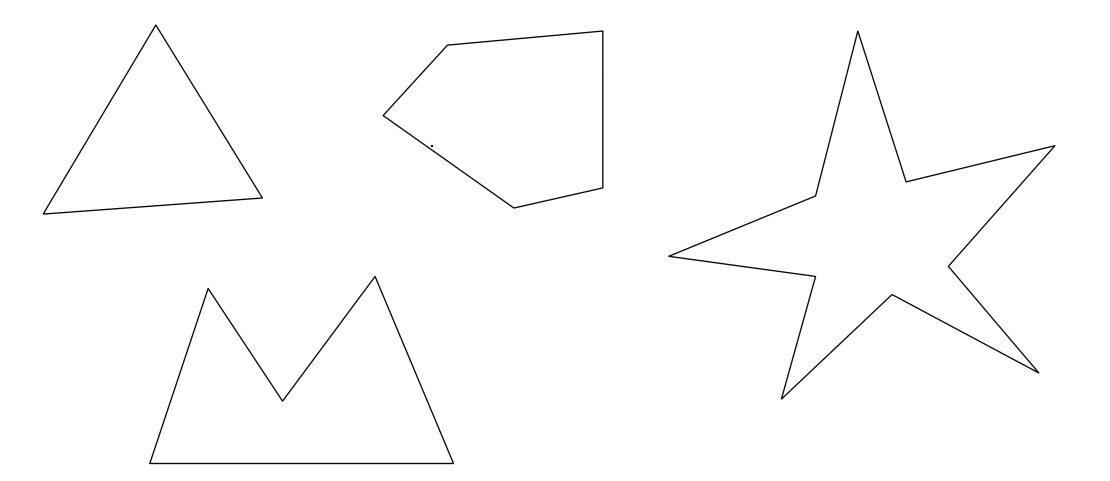
\includegraphics[scale=0.4]{Prosty}
  \caption{Przykłady wielokątów prostych}
  \label{fig:wielokat_prosty}
  \end{center}
\end{figure}

\begin{figure}[H]
  \begin{center}
  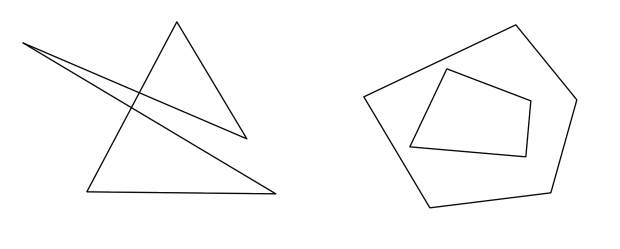
\includegraphics[scale=0.4]{Nieprosty}
  \caption{Przykłady wielokątów nieprostych}
  \label{fig:wielokat_nieprosty}
  \end{center}
\end{figure}

\subsubsection*{Wielokąt monotoniczny}

Wielokąt monotoniczny to taki wielokąt, dla którego możemy podać prostą $L$, taką że każda prosta prostopadła do niej przecina wielokąt w co najwyżej dwóch punktach (silna monotoniczność). Słabą monotonicznością nazywamy przypadek, gdy wielokąt posiada również krawędzie
prostopadłe do $L$. Na rysunku \ref{fig:wielokat_monotoniczny} dwa górne wielokąty są monotoniczne. Zielone proste mają jedno przecięcie z wielokątem, niebieskie – dwa, czerwone – trzy i więcej.

\begin{figure}[H]
  \begin{center}
  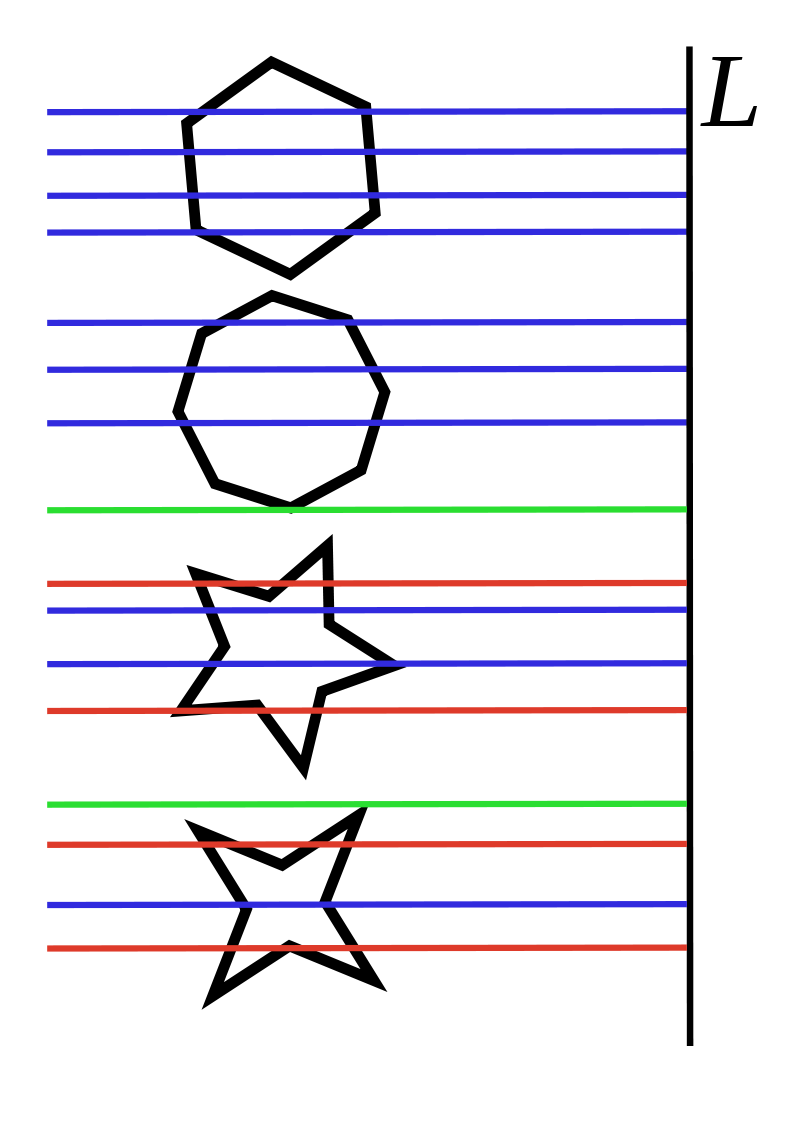
\includegraphics[scale=0.24]{Monotonic}
  \caption{Monotoniczność wielokątów (źródło: Wikipedia)}
  \label{fig:wielokat_monotoniczny}
  \end{center}
\end{figure}


\section*{Zadanie}

Podaj efektywny alogrytm do sprawdzenia czy dany $n$ kąt prosty jest monotoniczy względem podanej prostej (zadanie 10 na liście).
 
\section*{Algorytm}

Dowolny wielokąt i prostą $L$ możemy odpowiednio obrócić tak, żeby prosta $L$ była pionową oraz zostały zachowane wszystkie odległości między wierzchołkami wielokąta a prostą.

\begin{figure}[H]
  \begin{center}
  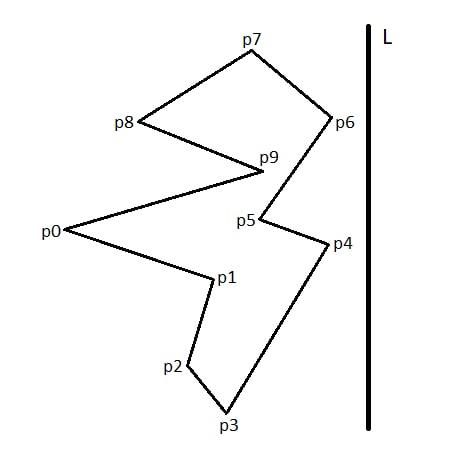
\includegraphics[scale=0.7]{Sample}
  \caption{Egzemplarz problemu}
  \label{fig:sample}
  \end{center}
\end{figure}

Żeby sprawdzić, czy dany $n$-kąt prosty jest monotoniczny względem prostej pionowej $L$, można zastosować następujący algorytm:

\begin{enumerate}
    \item Szukamy najwyższego punktu $p$ ($p_7$ na rysunku \ref{fig:sample} )
    \item Idziemy po kolejnych punktach w dół dopóki współrzędna $y$ danego punktu jest większa od $y$ następnego punktu (punkt końcowy $q = p_3$). Możemy poruszać się zgodnie z ruchem
    wskazówek zegara lub w przeciwnym kierunku, nie ma to znaczenia.
    \item Od punktu $q$ idziemy w góre, dopóki współrzędna $y$ danego punktu jest mniejszy od $y$ następnego punktu.
    \item Niech $m$ będzie liczbą odwiedzonych punktów w krokach 2 i 3. Jeśli $n = m$, to wielokąt jest silnie monotoniczny względem prostej $L$
\end{enumerate}

Jeżeli chcemy też uwzględnić słabą monotoniczność, to wystarczy przyjąć w korokach 2 i 3 że $y$ danego punktu może też być równy $y$ punktu następnego.

\subsection*{Analiza poprawności algorytmu}

Jeżeli $m < n$, to istnieje prosta pozioma, prostopadła do $L$, która przecina boki $(p_{m-1}, p_{m})$ oraz $(p_{m-2}, p_{m-1})$. A ponieważ przechodzenie po punktach zaczyna się od punktu najwyższego (czyli $y$ punktu $p_m$ jest mniejszy lub równy od $y$ punktu $p$), to wiemy
że na przeciwnej stronie wielokąta musi być jeszcze jeden bok, przecinający się z tą samą prostą poziomą, co znaczy że są 3 punkty przecięcia, a więc wielokąt nie jest monotoniczny. Jeżeli $m = n$, to takich przypadków nie istnieje.


\subsection*{Złożoność obliczeniowa}

Złożoności wszystkich etapów algorytmu:
\begin{itemize}
    \item Obrócenie wielokąta: $O(n)$
    \item Szukanie najwyższego punktu (krok 1, przeszukiwanie binarne): $O(log(n))$
    \item Przejście przez wierzchołki (krok 2 i 3): $O(n)$
\end{itemize}
Otóż złożoność całego algorytmu jest $O(n)$.

\end{document}
